% !TEX program = xelatex
%% Requires compilation with XeLaTeX or LuaLaTeX
\documentclass[10pt,xcolor={table,dvipsnames},t]{beamer}
\usepackage{biblatex}
\usepackage{caption}
\setbeamertemplate{caption}[numbered]
\addbibresource{reference.bib}
\usepackage{hyperref}
\hypersetup{ 
pdfpagemode=FullScreen,  
colorlinks=true,linkcolor=blue}
\usepackage{enumerate}

\usepackage{listings}
\usepackage{xcolor}

\definecolor{codegreen}{rgb}{0,0.6,0}
\definecolor{codegray}{rgb}{0.5,0.5,0.5}
\definecolor{codepurple}{rgb}{0.58,0,0.82}
\definecolor{backcolour}{rgb}{0.95,0.95,0.92}

\lstdefinestyle{mystyle}{
    backgroundcolor=\color{backcolour},   
    commentstyle=\color{codegreen},
    keywordstyle=\color{magenta},
    numberstyle=\tiny\color{codegray},
    stringstyle=\color{codepurple},
    basicstyle=\ttfamily\footnotesize,
    breakatwhitespace=false,         
    breaklines=true,                 
    captionpos=b,                    
    keepspaces=true,                 
    numbers=left,                    
    numbersep=5pt,                  
    showspaces=false,                
    showstringspaces=false,
    showtabs=false,                  
    tabsize=2
}

\lstset{style=mystyle}

% Flow chart config
\usepackage{tikz}
\usetikzlibrary{calc,trees,positioning,arrows,fit,shapes,calc}
\usetikzlibrary{shapes.geometric, arrows}
\tikzstyle{startstop} = [rectangle, rounded corners, minimum width=3cm, minimum height=1cm,text centered, draw=black, fill=red!30]
\tikzstyle{io} = [trapezium, trapezium left angle=70, trapezium right angle=110, minimum width=3cm, minimum height=1cm, text centered, draw=black, fill=blue!30]
\tikzstyle{process} = [rectangle, minimum width=3cm, minimum height=1cm, text centered, draw=black, fill=orange!30]
\tikzstyle{decision} = [diamond, minimum width=3cm, minimum height=1cm, text centered, draw=black, fill=green!30]
\tikzstyle{arrow} = [thick,->,>=stealth]

\usetheme{UCBerkeley}

\title[Your Short Title]{STMC coding team Training}
\subtitle{Lesson 3: Conditional statement}
\author{Tsai Yun Chen}
%\institute{}
\date{\today}

\begin{document}

\begin{frame}
  \titlepage
\end{frame}

% Uncomment these lines for an automatically generated outline.
%\begin{frame}{Outline}
%  \tableofcontents
%\end{frame}

\section{Class Goal}

\begin{frame}{Goal today}

\begin{itemize}
  \item Conditional statement \texttt{if}
  \item Comparison operators \texttt{==}, \texttt{!=} \texttt{>}, \texttt{<}, \texttt{<=}, \texttt{>=}
  \item More conditional statements \texttt{elif}, \texttt{else}
  \item Truth table, Boolean operators $\land$, $\lor$, $\neg$
\end{itemize}

\end{frame}


\section{Making decisions}
\begin{frame}{Making decisions}
    \begin{itemize}
      \item Sometimes we want a program to not only compute values, but also to \textit{make decisions}
      \vspace{2mm}
      \item How do we make decisions? Let's consider the simplest case:
      \begin{itemize}
        \item We ask a true or false question (e.g. Is it raining today?)
        \item We look at the answer of the question and act differently if the answer is true or false (e.g. It is raining today $\rightarrow$ not go out; It's not raining  $\rightarrow$ Go out )
      \end{itemize}
      \item We shall depict such relationship as follows:
    \end{itemize}
\end{frame}

\begin{frame}{Making decision: Flow chart}
  \begin{figure}
    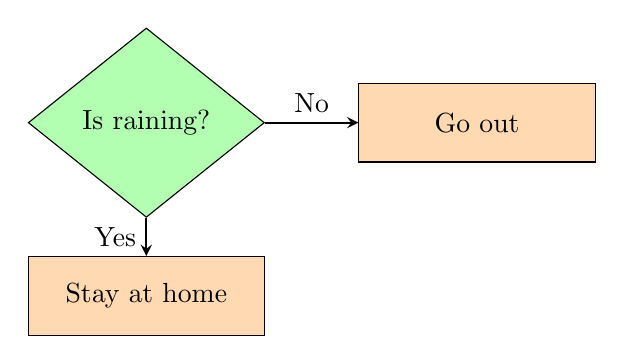
\begin{tikzpicture}[node distance=1.2cm]
      \node (dec1) [decision] {Is raining?};
      \node (no) [process, right of=dec1,xshift=3cm] {Go out};
      \node (yes) [process, below of=dec1,yshift=-1cm] {Stay at home};
      \draw [arrow] (dec1) -- node[anchor=east] {Yes} (yes);
      \draw [arrow] (dec1) -- node[anchor=south] {No} (no);

    \end{tikzpicture}
  \end{figure}
\end{frame}

\begin{frame}{Exercise}
  Before writing actual programs, let's exercise our thinking with flow charts. Draw a flow chart for a program that:
  \begin{itemize}
    \item Recieve two numbers $a,b$ as input and print out the larger number. Return either $a$ or $b$ if $a=b$.
    \item Reads body temperature $T$ from the user and prompt \texttt{"Fever"} if $T>38.0$
    \item Takes in an age $A$ and prompt \texttt{"valid"} if $3 \leq A \leq 100$. Otherwise print \texttt{"invalid"}
   \end{itemize}  
\end{frame}

\section{Boolean expressions}
\begin{frame}{Boolean expressions}
  \begin{itemize}
    \item As illustrated above, we need be able to ask questions in order to make decisions
    \item In python, ask questions with an \textbf{boolean expression} that return \textit{true} or \textit{false} depending on the evaluated answer
    \item For example of boolean expressions are:
    \begin{itemize}
      \item Is x > y ?
      \item Is x equal to y?
      \item etc.
    \end{itemize}
    \item Let's look at some examples to see how exactly can we do that in Python
  \end{itemize}
\end{frame}

\section{Comparision operators}

\begin{frame}{Equal to \texttt{==}}
  \begin{itemize}
    \item The operator \texttt{==} is the operator for \textbf{equal to}
    \item \textbf{Do not confuse it with a single =}
    \item \texttt{x==y} checks if x is equal to y
    \item An example of the so called \textit{comparsion operators}
    \item Examples:
    \begin{itemize}
      \item \texttt{1 == 0} $\rightarrow$ \texttt{false}
      \item \texttt{3 == 3} $\rightarrow$ \texttt{true}
      \item \texttt{'a' == 'A'} $\rightarrow$ \texttt{false}
      \item \texttt{'b' == 'b'} $\rightarrow$ \texttt{true}
    \end{itemize}
  \end{itemize}
\end{frame}
\begin{frame}[fragile]{Equal to \texttt{==}}
  \begin{itemize}
    \item We can also compare variables. For example
  \end{itemize}
\begin{lstlisting}[language=python]
age = int(input('Enter your age: '))
print(age == 14) # Should return True if age equals to 14
\end{lstlisting}
\begin{itemize}
  \item Another example
\end{itemize}
\begin{lstlisting}[language=python]
fatherAge = int(input('Father age: '))
motherAge = int(input('Mother age: '))
print(fatherAge == motherAge) 
# True only if fatherAge equals motherAge
\end{lstlisting}
\end{frame}
\begin{frame}[fragile]{Equal to \texttt{==}}
  \begin{itemize}
    \item Similarly we can do that for string
  \end{itemize}
\begin{lstlisting}[language=python]
yourName = input('What is your name: ')
print('yourName is:',yourName)
print(yourName == 'James') # Try inputing 'james', 'jAmEs' etc.
\end{lstlisting}
\begin{itemize}
  \item Another example
\end{itemize}
\begin{lstlisting}[language=python]
password = input('Enter password: ')
print(password == 'L^Enb2%') 
# You can imagine checking password this way might not be safe, to enhance safty people use hashing
\end{lstlisting}
\end{frame}

\begin{frame}{Larger than \texttt{>} or smaller than \texttt{<}}
  \begin{itemize}
    \item Similarly, we have \texttt{x > y} and \texttt{x < y}
    \item Checks if x is strictly larger than y or strictly smaller than y
    \item Example:
    \begin{itemize}
      \item \texttt{1.2 < 3.7} $\rightarrow$ \texttt{true}
      \item \texttt{0 < 1} $\rightarrow$ \texttt{false}
      \item \texttt{3 > 1} $\rightarrow$ \texttt{true}
      \item \texttt{9.9 > 3.7} $\rightarrow$ \texttt{true}
      \item \texttt{3 < 3} $\rightarrow$ \texttt{false} 
    \end{itemize}
  \end{itemize}
\end{frame}

\begin{frame}[fragile]{Larger than \texttt{>} or smaller than \texttt{<}}
  \begin{itemize}
    \item Some examples:
  \end{itemize}
\begin{lstlisting}[language=python]
examScore = float(input('Exam score: '))
print(examScore > 50.0) # True if examScore greater or equal to 50.0
\end{lstlisting}
\begin{itemize}
  \item Some more examples
\end{itemize}
\begin{lstlisting}[language=python]
integer = int(input('Enter integer: '))
print(integer < 0) # True if it's negative number
\end{lstlisting}
\end{frame}

\begin{frame}{More operators: \texttt{>=}, \texttt{<=}, \texttt{!=}}
  \begin{itemize}
    \item Similarly, we also have \textbf{smaller than or equal to} \texttt{<=} and \textbf{larger than or equal to} \texttt{>=}
    \item Examples
    \begin{itemize}
      \item \texttt{1 >= 1} $\rightarrow$ \texttt{true}
      \item \texttt{3 >= 1} $\rightarrow$ \texttt{true}
      \item \texttt{4 <= 1} $\rightarrow$ \texttt{false}
    \end{itemize}
    \item We also have \textbf{not equal to} \texttt{!=}
    \item  Examples:
    \begin{itemize}
      \item  \texttt{1 != 1} $\rightarrow$ \texttt{false}
      \item  \texttt{3 != 2} $\rightarrow$ \texttt{true}
      \item  \texttt{'a' != 'a'} $\rightarrow$ \texttt{false}
      \item  \texttt{'a' != 'A'} $\rightarrow$ \texttt{true}
    \end{itemize}
  \end{itemize}
\end{frame}
\begin{frame}[fragile]{More operators: \texttt{>=}, \texttt{<=}, \texttt{!=}}
\begin{itemize}
  \item Some examples:
\end{itemize}
\begin{lstlisting}[language=python]
timHeight = float(input('Height of Tim: '))
mayHeight = float(input('Height of May: '))
print(timHeight <= mayHeight) # True if Tim's height is less than or equal to May's
\end{lstlisting}
\begin{itemize}
  \item Another example:
\end{itemize}
\begin{lstlisting}[language=python]
number1 = int(input('Enter a number: '))
number2 = int(input('Enter another number: '))
print(number1 != number2) # True if the two are not the same  
\end{lstlisting}
\end{frame}

\section{If statement}
\begin{frame}[fragile]{\texttt{if} statement}
  \begin{itemize}
    \item Now we know how to ask questions. Let's see how we can make decision
    \item In python decisions are made using \textbf{conditional statement}
    \item One simplest type is the \texttt{if} statement. Here is the syntax:
\begin{lstlisting}[language=python]
  if """boolean expression""":
    # Run if true
\end{lstlisting}
    \item Note that you must \textbf{indent the after if. Otherwise error will be raised}
  \end{itemize}
\end{frame}

\begin{frame}[fragile]{\texttt{if} statement}
  Example:
\begin{lstlisting}[language=python]
# This code checks if a number is negative
number = int(input('Enter a number: '))

if number < 0:
  print('This is negative!') # Make sure to indent!

print('This will always be run') # This will always be run
\end{lstlisting}
Draw the flowchart of the code above
\end{frame}
\begin{frame}{\texttt{if} statement}
  \begin{exampleblock}{Exercise (Password checking):}
    Make up a password. Write a program that reads in a string \texttt{password} and check it against your made up password. Print \texttt{Login successful} if the password is correct and print nothing otherwise.
  \end{exampleblock}
  \begin{exampleblock}{Exercise (Password checking 2):}
    Modify the code. Print \texttt{Login success} if successful and \texttt{Login failed} otherwise
  \end{exampleblock}
\end{frame}
\section{if-else statement}
\begin{frame}[fragile]{\texttt{if-else} statement}
  \begin{itemize}
    \item As shown in previous examples, we can definitely use two if statements to check otherwise
    \item However, \texttt{True} and \texttt{not True} are \textbf{mutually exclusive}. That is, they cannot happen at the same time. So the \textit{second checking is redudant}
    \item To introduce a more effcient way to do it, we introduce the \texttt{if-else} statement. Here is the syntax:
  \end{itemize}
\begin{lstlisting}[language=python]
if """condition""":
  # If True run here
else:
  # Otherwise run here
\end{lstlisting}
\end{frame}
\begin{frame}[fragile]{\texttt{if-else} statement}
Some examples:
\begin{lstlisting}[language=python]
# Compare height
timHeight = float(input('Tim\'s height: '))
mayHeight = float(input('May\'s height: '))
if timHeight > mayHeight:
  print('Tim is taller')
else:
  print('May is taller or they have same height')
\end{lstlisting}
Again draw a flowchart of the code
\end{frame}


% \begin{frame}{\texttt{if-else} statement}
%   \begin{exampleblock}{Exercise:}
%     John is a middle schooler. Everyday he can either be happy or unhappy. If he is happy, he will study; If he is not, he will play computer games. Let \texttt{happiness} be John's happiness. If \texttt{happiness} is 1, he is happy; otherwise, he is not. Write a program that predicts what John will do given his happiness.
%   \end{exampleblock}
%   \vspace{1mm}
%   \textbf{Input:} An integer \texttt{happiness} which is either 0 or 1\\
%   \textbf{Output:} Print "He will study" if he is happy and "He will play computer games" if not.
% \end{frame}

% \begin{frame}[fragile]{\texttt{if-else} statements}
%   \begin{exampleblock}{Exercise: Rainstorm signal}
%     \begin{columns}
%       \column{0.7\textwidth}
%       According to HKO, the Black rainstorm signal is issued if the hourly rainfall exceeds 70mm. Write a program that takes in the hourly rainfall \texttt{rainfall} in mm and determine whether the black rainstorm signal is issued. Return \texttt{BLACK} if so and \texttt{OTHERS} if otherwise. 
%       \column{0.2\textwidth}
%       \begin{figure}
%         
\includegraphics{img/black-rain.png}
%         \caption*{Source: \href{https://www.hko.gov.hk/en/wservice/warning/rainstor.htm}{HKO}}
%       \end{figure}
%     \end{columns}
%   \end{exampleblock}
%   \textbf{Example Input/output}
% \begin{lstlisting}[language=bash]
%     Example 1:      Example 2:      Example 3:      Example 4:
%     $./main         $./main         $./main         $./main
%     0               70.0            72.4            23.1
%     OTHERS          OTHERS          BLACK           OTHERS
% \end{lstlisting}
% \end{frame}


\begin{frame}[fragile]{\texttt{if-else} statement}
  \begin{exampleblock}{Exercise: Overbudget}
    Merry has \$300 dollar in her pocket. Since Christmas is approaching, she decided to buy some gifts for her friends. The types of gifts she wanted to buy are: Pencil (\$3.0 each), Cake (\$11.0 each) and Book (\$ 80.0 each). Suppose she bought $a$ pencil,  $b$ books and $c$ cake. Write a program to determine whether she exceeded her budget. If no, print \texttt{NO OVERBUDGET}; otherwise, print \texttt{EXCEEDED <amount>}.
  \end{exampleblock}
\begin{lstlisting}[language=bash]
  Example 1:            Example 2:        Example 3:
  101                   1                 5
  0                     27                4
  0                     0                 3
  EXCEEDED 3.000000     NO OVERBUDGET     NO OVERBUDGET    
\end{lstlisting}
\end{frame}
\section{nested if statement}
\begin{frame}[fragile]{Nested \texttt{if} statement}
  \begin{itemize}
    \item Some times we want to test for more cases at once before outputing otherwise
    \item In those cases we might want to follow \texttt{else} with another \texttt{if}. 
    \item We called that a \textbf{nested conditional statement} For example:
\begin{lstlisting}[language=python]
if """condition""":
  # Condition 1 True 
else:
  if """condition 2""":
    # Condition 1 False but Condition 2 True
  else:
    # Condition 1 and Condition 2 both False
\end{lstlisting}
  \end{itemize}
  Again, remember to \textbf{indent twice for the nested statement}
\end{frame}

% \begin{frame}[fragile]{More decisions}
%   \begin{exampleblock}{Exercise: Rainstorm signal+}
%     According to HKO, the amber, red and black rainstorm signal is issued if the hourly rainfall exceed 30mm, 50mm and 70mm respectively (inclusive). Write a program that takes in a float \texttt{rainfall} and return \texttt{AMBER}, \texttt{RED} or \texttt{BLACK} accordingly if there's a signal, and \texttt{NO SIGNAL} if there is no signal. Furthermore, return \texttt{ERROR} if \texttt{rainfall} < 0.
%   \end{exampleblock}
% \begin{lstlisting}[language=bash]
%   Example 1:      Example 2:      Example 3:      Example 4:
%   $./main         $./main         $./main         $./main
%   0               70.0            53.4            30.2
%   NO SIGNAL       BLACK           RED             AMBER

%   Example 5:
%   $./main
%   -3
%   ERROR
% \end{lstlisting}
% \end{frame}

\section{if-elif-else statement}
\begin{frame}[fragile]{\texttt{if-elif-else} statements}
  \begin{itemize}
    \item Sometimes, nested statements can be messy
    \item Luckily, python provide another way to implement \texttt{else} followed by \texttt{if}
    \item We introduce the \texttt{elif} (\textit{else-if}), which has the following syntax
  \end{itemize}
\begin{lstlisting}[language=python]
if """Condition 1""":
  # If 1 is true
elif """Condition 2""": # Check if 1 is false 
  # If 2 is true
else:
  # If both 1 and 2 are false
\end{lstlisting}
\end{frame}

\begin{frame}[fragile]{\texttt{if-elif-else} statement}
  \begin{itemize}
    \item Of course, there are multiple variants of such statement. 
    \item For example, if you don't want to do anything if both 1 and 2 are false:
  \end{itemize}
\begin{lstlisting}[language=python]
if """condition 1""":
  # If 1 is true 
elif """condition 2""":
  # If 1 false and 2 true
# No else here, so do nothing when both are false
\end{lstlisting}
\end{frame}

\begin{frame}[fragile]{\texttt{if-elif-else} statement}
  \begin{itemize}
    \item Similarly, you can stack them together if you want to check a lot of cases
  \end{itemize}
\begin{lstlisting}[language=python]
if """condition 1""":
  # 1 is true
elif """condition 2""":
  # 2 is true, 1 is false
elif """condition 3""":
  # 3 is true, 1 and 2 are false
elif """condition 4""":
  # 4 is true, 1 and 2 and 3 are false 

# You can continue to stack as many cases as you like
\end{lstlisting}
\end{frame}

\begin{frame}[fragile]{\texttt{if-elif-else} statement}
  Some examples:
\begin{lstlisting}[language=python]
# Compare height
timHeight = float(input('Tim\'s height: '))
mayHeight = float(input('May\'s height: '))
if timHeight > mayHeight:
  print('Tim is taller')
elif mayHeight > timHeight:
  print('May is taller')
else:
  print('They have the same height')
\end{lstlisting}
  Again draw a flowchart of the code
\end{frame}

\begin{frame}[fragile]{\texttt{if-elif-else}}
  \begin{exampleblock}{Exercise: Grading program}
    We shall write a grading program. Take a \texttt{score} as input and print out a grade according to the following table:
    \begin{table}[]
      \begin{tabular}{ll}
      Score ($s$)      & Grade \\
      $85< s \leq 100$ & A     \\
      $70< s \leq 85$  & B     \\
      $55< s \leq 70$  & C     \\
      $40< s \leq 55$  & D     \\
      $s<40         $  & F
      \end{tabular}
      \end{table}
  \end{exampleblock}
\end{frame}

\section{Boolean operators}
\begin{frame}{Boolean expression}
  \begin{itemize}
    \item Recall \textbf{boolean expression} is an expression that \textbf{either returns true or false}
    \item Examples:
    \begin{itemize}
      \item "John has beard"
      \item "Spiders more than 2 legs"
      \item "x is equal to y"
      \item "There is more sand on the Earth than stars on the universe"
    \end{itemize}
    \item Now we want to \textit{combine} or \textit{modify} these expressions
  \end{itemize}
\end{frame}

\begin{frame}{Combining expressions}
  \begin{itemize}
    \item Let's consider how boolean expressions can be combined
    \item Consider the statements:
    \begin{enumerate}
      \item Today is raining
      \item Eva has an umbrella
    \end{enumerate}
    \item One way to combine them is to use the connective "and"
    \item So we have "Today is raining and Eva has an umbrella"
    \item Now, when is the new statement true? (i.e. suppose we were to put it inside a if statement, when should the if statement fire)
  \end{itemize}
\end{frame}

\begin{frame}{Combining expression}
  We can investigate the problem by using a \textbf{truth table}
  \begin{table}[]
    \begin{tabular}{ccc}
    Today is raining & Eva has an umbrella & Today is raining and Eva has an umbrella \\
    T                & T                   & T                                        \\
    T                & F                   & F                                        \\
    F                & T                   & F                                        \\
    F                & F                   & F                                       
    \end{tabular}
    \end{table}
    We can see that the final statement "Today is raining and Eva has an umbrella" is true only if \textit{both} "Today is raining" and "Eva has an umbrella" are individually true
\end{frame}

\begin{frame}{Combining expression}
  \begin{itemize}
    \item In fact, we can see the above table is not limited to "Today is raining" and "Eva has an umbrella"
    \item For any boolean expression $a$, $b$, we can always combine $a$,$b$ by asking if $a$ and $b$ is true
    \item Hence, the truth table above define the operation "and"
    \item Let's define different operations together
  \end{itemize}
\end{frame}

\subsection{AND Operator}

\begin{frame}{Logical AND $\land$}
  \begin{columns}
    \column{0.6\textwidth}
    \begin{itemize}
      \item The \textbf{logical AND} $\land$ is a binary operation
      \item It combines two statements $a,b$ and return true only if \textit{both} statements are true 
      \item In python this is done using the \texttt{and} keyword
      \item Example:
      \begin{itemize}
        \item \texttt{1 <= var and var < 3} 
        \item \texttt{(number \% 3 == 0)  and (number \% 2 != 0)}
        \item \texttt{(chr != 'A') and (chr != 'B')}
      \end{itemize}
    \end{itemize}
    \column{0.4\textwidth}
    \begin{table}[]
      \begin{tabular}{ccc}
      $a$ & $b$ & $a\land b$  \\
      T & T & T \\
      F & F & F \\
      F & T & F\\
      T & F & F
      \end{tabular}
      \caption{Truth table of $\land$}
      \end{table}
  \end{columns}
\end{frame}

\begin{frame}[fragile]{Logical AND $\land$}
  \begin{itemize}
    \item For example:
  \end{itemize}
\begin{lstlisting}[language=python]
username = input('Username: ')
password = input('Password: ')
if username == 'animal' and password == 'elephant': 
  print('Login success')
else:
  print('Login failed')
# P.S. Don't use this kind of password in real life 
\end{lstlisting}
\end{frame}

\begin{frame}[fragile]{Logical AND $\land$}
  \begin{itemize}
    \item Another example:
  \end{itemize}
\begin{lstlisting}[language=python]
age = int(input('Enter age: '))
if 0 < age and age < 120:
  print('This age make sense')
else:
  print('This age does not make sense')
\end{lstlisting}
\end{frame}


\subsection{OR operator}
\begin{frame}{Logical OR $\lor$}
  \begin{columns}
    \column{0.6\textwidth}
    \begin{itemize}
      \item The \textbf{logical OR} $\lor$ is a binary operation
      \item It combines two statements $a,b$ and return true only if \textit{either} of the statements are true 
      \item In python, this is done using \texttt{or} keyword
      \item Example:
      \begin{itemize}
        \item \texttt{(var == 1) or (var == 2)}
        \item \texttt{count > 1 or count < -1}
        \item \texttt{(var == 1) or (var != 3)}
      \end{itemize}
    \end{itemize}
    \column{0.4\textwidth}
    \begin{table}[]
      \begin{tabular}{ccc}
      $a$ & $b$ & $a\lor b$  \\
      T & T & T \\
      F & F & F \\
      F & T & T\\
      T & F & T
      \end{tabular}
      \caption{Truth table of $\lor$}
      \end{table}
  \end{columns}
\end{frame}

\begin{frame}[fragile]{Logical OR $\lor$}
  \begin{itemize}
    \item Some examples:
  \end{itemize}
\begin{lstlisting}[language=python]
instru = input('What musical instruments you like? ')

if instru == 'guitar' or instru == 'bass':
  print('So you like string instruments!')

elif instru == 'brass' or instru == 'trumpet':
  print('So you like wind instruments!')

else:
  print('Sorry, I don\'t know what is ',instru)
\end{lstlisting}
\end{frame}

\begin{frame}[fragile]{Logical OR $\lor$}
  \begin{itemize}
    \item Another example that combines \texttt{and} with \texttt{or}
  \end{itemize}
\begin{lstlisting}[language=python]
# Tickets are sold only to kids from age 8 to 15 or elderly from age 60-80
age = int(input('Enter you age: '))

if (8 <= age and age <= 15) or (60 <= age and age <= 80):
  print('You are eligible')
else:
  print('Nope, you cannot buy this')
\end{lstlisting}
\end{frame}

\subsection{NOT operator}
\begin{frame}{Negation operation $\neg$}
  \begin{columns}
    \column{0.6\textwidth}
    \begin{itemize}
      \item The \textbf{negation operation} $\neg$ is a unitary operation 
      \item It is equivalent to adding "not" to the statement 
      \item In python, this is done by adding \texttt{not} in front of conditionals
      \item Example:
      \begin{itemize}
        \item \texttt{not(var > 3)} $\leftrightarrow$ \texttt{(var <= 3)}
        \item \texttt{not(var == 3)} $\leftrightarrow$ \texttt{(var != 3)}
      \end{itemize}
    \end{itemize}
    \column{0.4\textwidth}
    \begin{table}[]
      \begin{tabular}{cc}
      $a$ & $\neg a$  \\
      T & F \\
      F & T
      \end{tabular}
      \caption{Truth table of $\neg$}
      \end{table}
  \end{columns}
\end{frame}

\begin{frame}[fragile]{Negation operation $\neg$}
  \begin{itemize}
    \item Some examples
  \end{itemize}
\begin{lstlisting}[language=python]
# Today (5/11) is the open day of HKUST (for real)
# There are events that bring visitors to visit different labs
# However these event should only open to student that are not already the student of HKUST

school=input('Which school do you belongs to? ')

if not (school=='HKUST'):
  print('welcome to the event')
else:
  print('you are already a student of HKUST')
\end{lstlisting}
\end{frame}

\begin{frame}[fragile]{Summary Exercise}
  \begin{enumerate}
    \setcounter{enumi}{2}
    \item Every year that is exactly divisible by four is a leap year, except for years that are exactly divisible by 100, but these centurial years are leap years if they are exactly divisible by 400. For example, the years 1700, 1800, and 1900 are not leap years, but the years 1600 and 2000 are. Write a program that determines whether a year is a leap year.
  \end{enumerate}
  \begin{lstlisting}
  $./main             ./main              ./main
  1700                1600                2012
  Not leap year       Is leap year        Is leap year
  \end{lstlisting}
\end{frame}

\begin{frame}[fragile]{Summary Exercises}
  \begin{enumerate}
    \setcounter{enumi}{3}
    \item Write a program that reads in 3 numbers and ouput the largest number. You are guaranteed that no two numbers are equal. Expected ouput
\begin{lstlisting}[language=bash]
$./main
13 83 19
2nd number is largest. The value is 83

$./main
77 21 3
1st number is largest. The value is 77

$./main
0 21 88
3rd number is largest. The value is 88
\end{lstlisting}
  \end{enumerate}
\end{frame}

\begin{frame}[fragile]{Finally, Homework}
  \begin{itemize}
    \item Homework 2 is posted on the course website, namely the HW2.ipynb
    \item same as last time, 3 problems, sorted in ascending order of difficulty
    \item submit the homework to \href{https://drive.google.com/drive/folders/1TqSFSwu8-KdzIHZcQWB7PjgqPJen4dsO?usp=sharing}{the same place}, inside the folder of \texttt{HW2 submission}
    \item remember to include all your group member's name in the document
    \item deadline: before next lesson, i.e. 16/3
    \item the solution will be disclosed one week after the deadline, i.e. 23/3
    \item comment on HW1 will be given
  \end{itemize}
\end{frame}

\end{document}
